\smalltitle{سوال 1}
\begin{enumerate}
    \item به صورت کاردینالی به صورت زیر نشان داده می‌شود:
    \begin{figure}[H]
        \centering 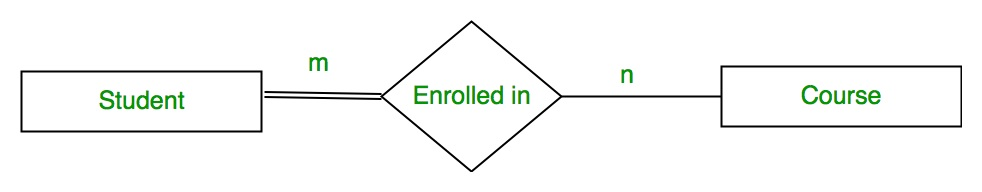
\includegraphics[scale=0.4]{pics/nullable1.jpg}
    \end{figure}
    دو خط که بین
    \lr{Student} و \lr{Course}
    نشان دهنده‌ی اختیاری بودن آن رابطه است. به عنوان مثال در اینجا این دیاگرام نشان دهنده‌ی این است
    که هر درس می‌تواند توسط تعدادی دانشجو اخذ شده باشد یا نه. این یعنی درسی می‌تواند خالی بماند.

    \noindent
    برای نشانه گذاری کمینه و بیشینه می‌توان به صورت زیر عمل کرد:
    \begin{figure}[H]
        \centering 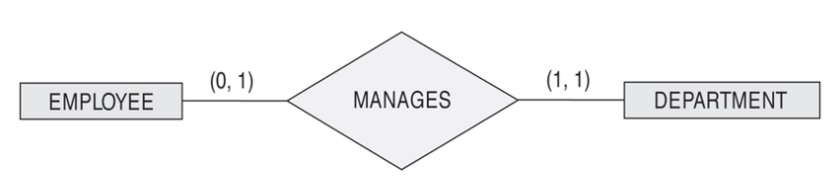
\includegraphics[scale=0.4]{pics/nullable2.jpg}
    \end{figure}
    در این مثال هر کارمند می‌تواند 1 یا 0 بخش را مدیریت کند ولی هر بخش حتما توسط یک نفر مدیریت می‌شود.
    \item \textbf{فایل}:
    \begin{enumerate}
        \item سادگی در ذخیره‌سازی فایل
    \end{enumerate}
    \textbf{پایگاه داده}:
    \begin{enumerate}
        \item کمتر کردن تکرار به کمک رابطه‌ها
        \item ارتباط تحت شبکه. این موضوع کمک می‌کند که برنامه‌ اصلی و دیتابیس را در دو کامپیوتر مختلف اجرا کنیم
        \item امکان درخواست (کوئری) زدن‌های پیچیده
        \item هندل کردن اتوماتیک \lr{data race} در خود دیتابیس
    \end{enumerate}
    \item رابطه‌ی دانشجو و دپارتمان
\end{enumerate}



